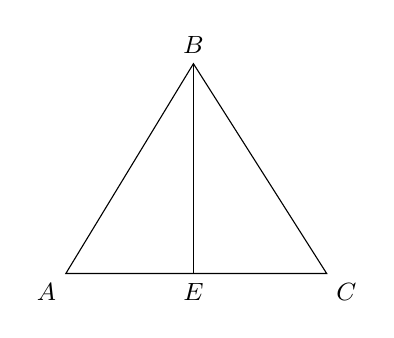
\begin{tikzpicture}[scale=.72, every node/.style={font=\small}]
  \coordinate (A) at (0,0); \coordinate (C) at (4.6,0); \coordinate (B) at (2.25,3.7); \coordinate (E) at (2.25,0);
  \draw (A)--(B)--(C)--cycle; \draw (B)--(E);
  \foreach \p/\pos in {A/below left,B/above,C/below right,E/below}
    \node[\pos] at (\p) {$\p$};
\end{tikzpicture}
